\newpage
\begin{flushleft}
  \textbf{\large 2 Обзор современных подходов к отслеживаю объектов на видеоизображениях}
\end{flushleft}
\refstepcounter{chapter}
\addcontentsline{toc}{chapter}{2 Обзор современных подходов к отслеживаю объектов на видеоизображениях}
В этой главе будут подобно рассмотрены следующие вещи:
\begin{itemize}
  \item[--] набор данных для сравнения различных алгоритмов друг с другом;
  \item[--] различные метрики, по которым проводится сравнение;
  \item[--] принцип работы и основные отличительные особенности выбранных алгоритмов. 
\end{itemize}
\section{Набор данных MOT17}
Набор данных MOTChallenge \cite{dendorfer2021motchallenge} является одним из наиболее популярных в области для сравнения между собой различных алгоритмов отслеживания нескольких объектов на видеоизображениях одновременно. 
Со дня своего появления он быстро обрел статус стандарта индустрии. 

Бенчмарк MOT17 был выпущен в 2017 году и является идейным наследником более ранних версий -- MOT15 и MOT16. В ходе этого развития авторами был исправлен ряд проблем старых версий:
\begin{itemize}
    \item[--] с развитием технологии отслеживания объектов на изображении MOT15 стал слишком простым для современных методов. MOT16 начал включать в себя ряд новых видео, где траектории объектов чаще пересекаются друг с другом, условия освещения более разнообразны, а средняя плотность объектов на изображении увеличилась в три раза;
    \item[--] MOT17 решает другую важную проблему -- уточняет разметку набора данных, так как в предыдущей версии нередко встречались ошибки. 
\end{itemize}

В итоге MOT17 включается в себя 14 различных видео общей протяженностью порядка 4 минут. Все они представляют из себя различные записи с уличных камер, на которых пешеходы перемещаются по тротуарам, площадям, торговым центрах. 
В наборе данных представлены различные ракурсы: как видео с подвижной камерой снятые человеком, находящимся в толпе, так и сделанные с возвышенности статично, например, камерой наблюдения.

На рисунках \ref{fig:mot_1}-\ref{fig:mot_3} приведены примеры изображений из бенчмарка.

\begin{figure}[ht]
    \centering
    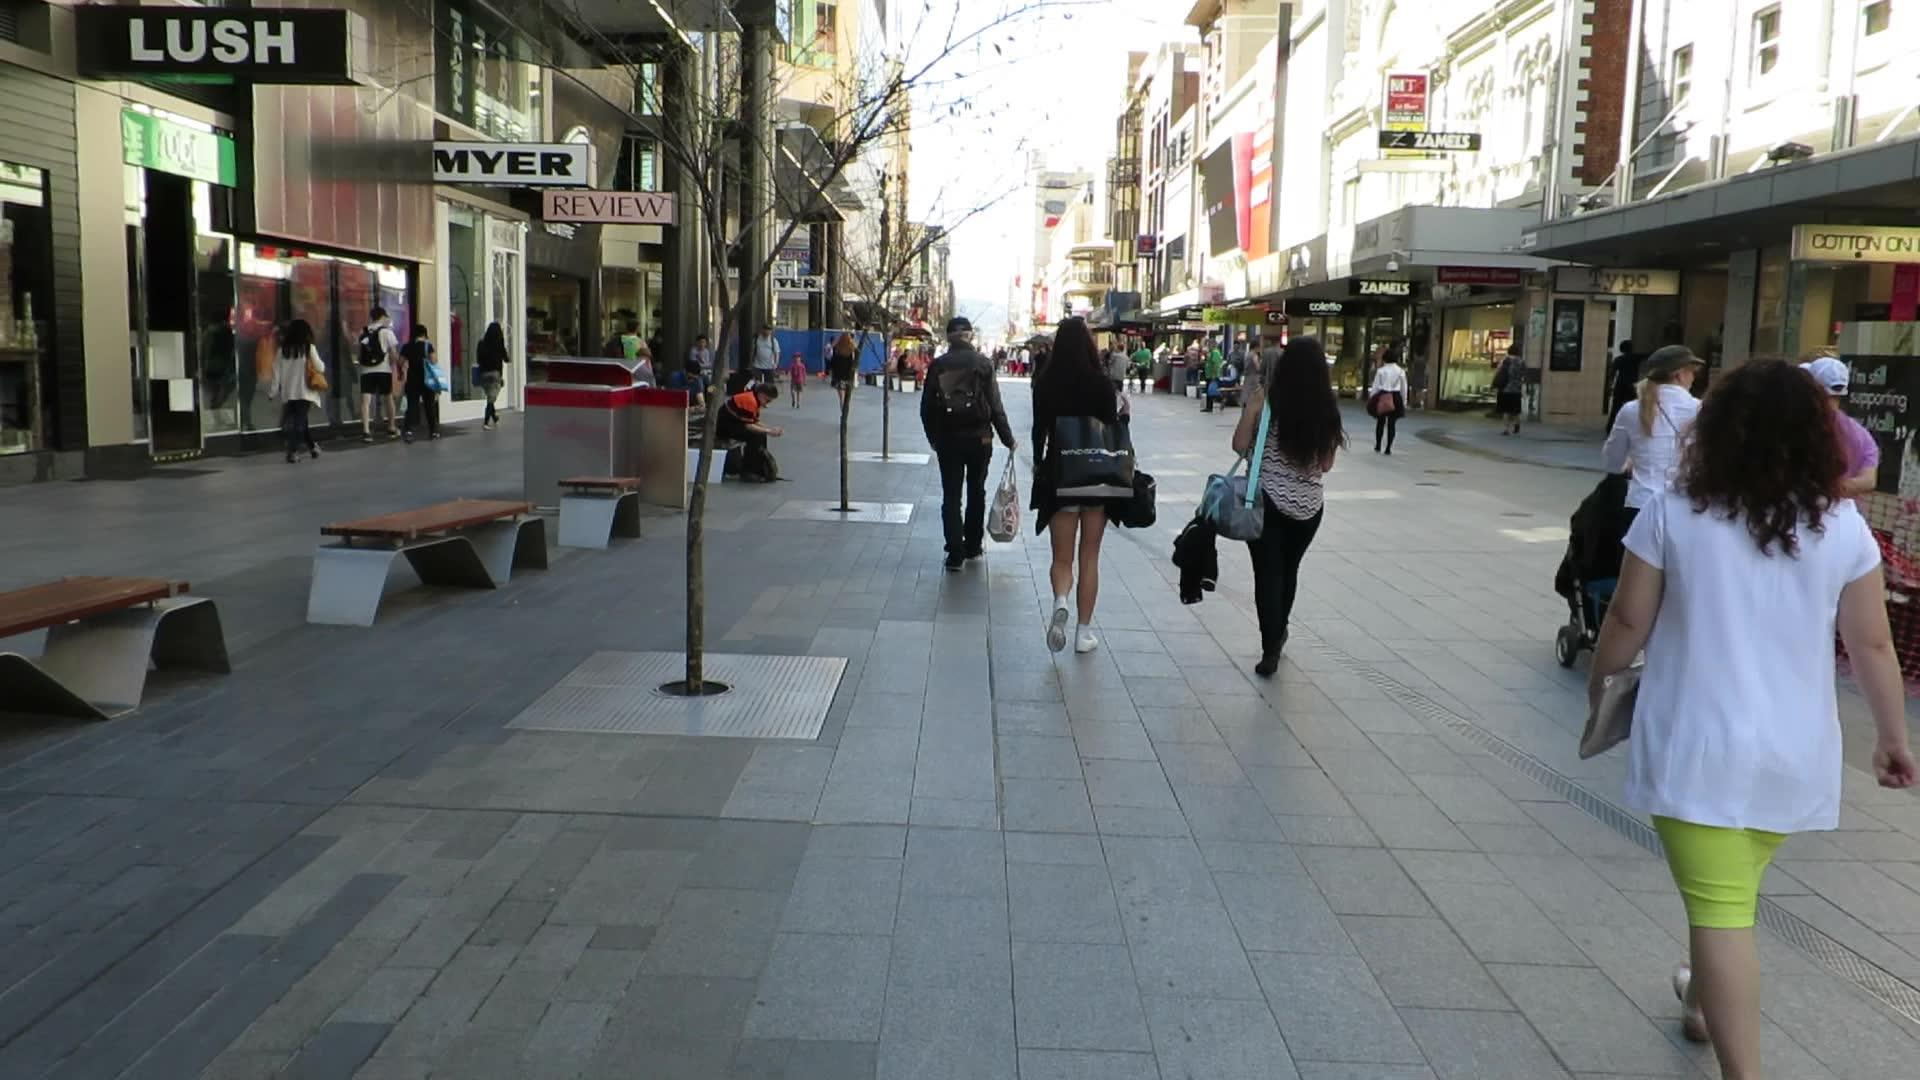
\includegraphics[width=0.7\textwidth]{review/MOT17_1}
    \caption{Пример изображения из набора данных MOT17 (приводится по \cite{dendorfer2021motchallenge}, страница 850, рисунок 3).}
    \label{fig:mot_1}
\end{figure}

\begin{figure}[ht]
    \centering
    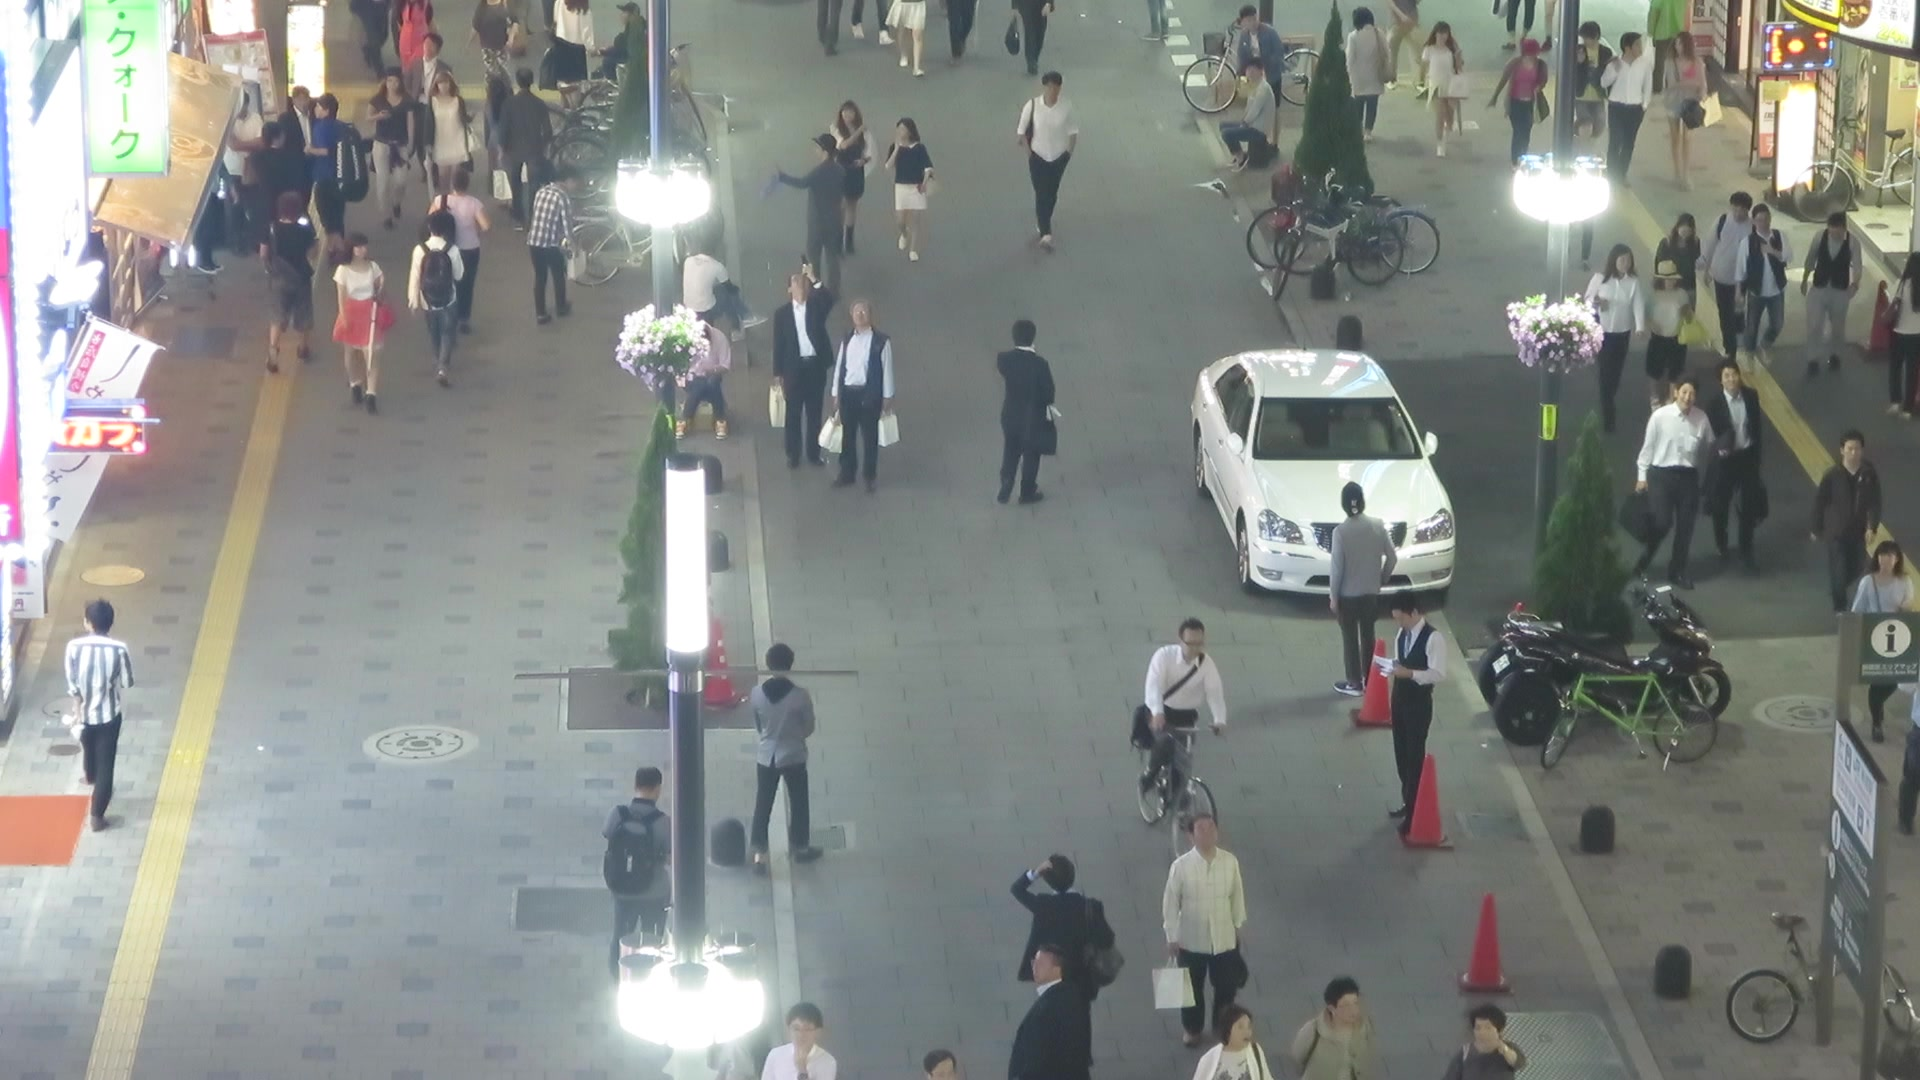
\includegraphics[width=0.7\textwidth]{review/MOT17_2}
    \caption{Пример изображения из набора данных MOT17 (приводится по \cite{dendorfer2021motchallenge}, страница 850, рисунок 3).}
    \label{fig:mot_2}
\end{figure}

\begin{figure}[ht]
    \centering
    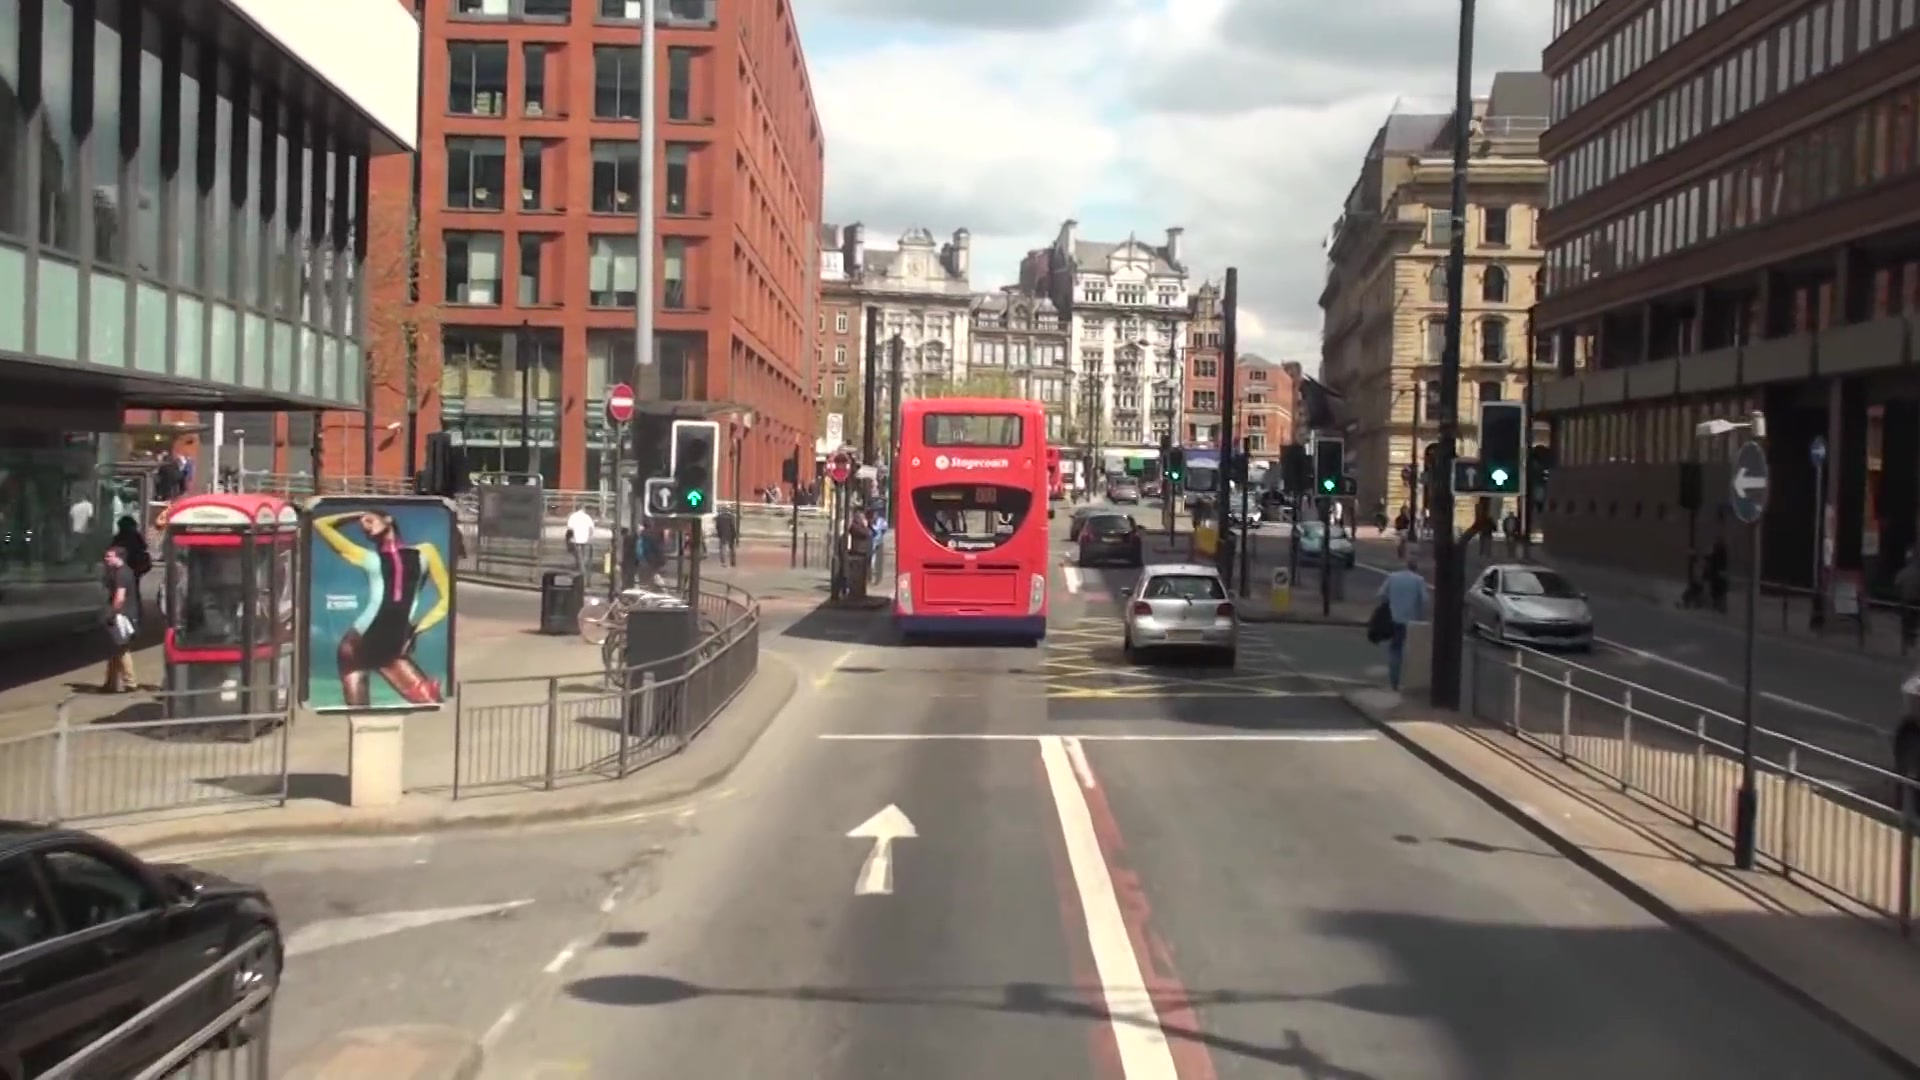
\includegraphics[width=0.7\textwidth]{review/MOT17_3}
    \caption{Пример изображения c из набора данных MOT17(приводится по \cite{dendorfer2021motchallenge}, страница 850, рисунок 3).}
    \label{fig:mot_3}
\end{figure}

\FloatBarrier
\section{Метрики для оценивания}
В этом разделе разбираются основные метрики для оценивания качества отслеживая объектов на видеоизображениях.
\subsection{Метрика MOTA}
Метрика МОТА\cite{bernardin2008evaluating} (англ. Multiple Object Tracking Accuracy -- точность отслеживания нескольких объектов) была предложена еще в 2008 году и является старейшей из всех используемых в работе. 
Ее авторы ставили целью создать критерий, который позволит оценивать точность выполнения задачи слежения. 
Подчеркивается важность способности метрики учитывать постоянство идентификации, точность оценки положения объекта и итоговой траектории.
Более того, был сделан акцент на минимизации параметров, а также интуитивной понятности для человека и применимости для задач слежения в любой постановке.

В итоге был предложен следующий способ вычисления 
\begin{equation}
    \text{MOTA} = 1 - \frac{\sum_{t=0}^{T}(\text{FP} + \text{FN} + \text{IDSW})}{\sum_{t=0}^{T}g_t},
    \label{eq:mota}
\end{equation}
где FP -- количество неверно найденных объектов, которые на самом деле не были отмечены на изображении при разметке; FN -- количество объектов, которые были отмечены при разметке, но не были найдены алгоритмом на изображении; 
IDSW -- сколько найденных ранее объектов не были правильно реидентифицированы и получили новый уникальный идентификационный номер, \(g_t\) -- общее количество объектов, отмеченных при разметке на кадре.
Из формулы \ref{eq:mota} видно -- чем больше показатель метрики, тем лучше справляется алгоритм.

Существует критика метрики MOTА, связанная с суммированием ошибок разного рода без какой-либо их предобработки, % \cite{dendorfer2021motchallenge}, 
а также плохой репрезентацией при отслеживании с использованием нескольких камер. % \cite{ristani2016performance}. 
Тем не менее, MOTA используется практически в каждом исследовании по теме и на практике доказала свою состоятельность в оценивании качества отслеживания объектов на видеоизображениях. Именно поэтому было принято решение включить ее в качестве критерия для сравнения методов в данной работе.
\subsection{Метрика IDF1}
Метрика IDF1 \cite{ristani2016performance} рекомендована для анализа производительности трекера в качестве дополнительно в связи с некоторым недостатками MOTA.

Авторы считали, что основная проблема других оценок -- арифметические операции с разнородными ошибками, которые могут оказывать влияние на интерпретируемость полученного результата. В общем, они оценивали вероятность появления ошибок идентификации и детектирования в каждый момент времени, а не точность итоговых траекторий у каждого объекта. 

Предложенная метрика IDF1 фокусировалась на оценке того, насколько качественно и долго трекер сохраняет идентичности объектов. Для этого, полученные с помощью трекера объекты, их идентичности и итоговые траектории сопоставляются с размеченными на основе методов графовой оптимизации, благодаря чему размеченные траектории сопоставляются с полученными на основе минимизации ошибки. Получившаяся оценка является более репрезентативной с точки зрения отслеживания конкретного объекта, так как оценивает именно задачу сохранения идентификации и точности итоговых траекторий.  
При этом у метрики есть и свои недостатки, поэтому авторы позиционирует ее как дополнительную для более комплексной оценки. 

Метрики IDF1 представляет из себя
\begin{equation}
    \label{eq:idf1}
    \text{IDF1} = \frac{2 \text{IDTP}}{2\text{IDTP} + \text{IDFP} + \text{IDFN}},
\end{equation}
где IDTP -- количество верно идентификационных отслеживаемых объектов; IDFN -- количество ненайденных объектов, которые были в разметке, но которым не были сопоставлены траектории; IDFP -- количество ложных срабатываний, когда был найден несуществующий объект. 
Расчет всех этих значений происходит после упомянутого ранее процесса сопоставления полученных траекторий с размеченными на основе оптимизации графа. 

% Полученная оценка является ед

В итоге, благодаря оценке с точки зрения качества сохранения присвоенных ранее идентификаций, метрика IDF1 является отличным дополнением для MOTA и была выбрана для учета в сравнении методов отслеживания объектов на видеоизображении в рамках данной работы.
\subsection{Метрика HOTA}
\cite{luiten2021hota}

\section{Обзор существующих алгоритмов }
Тут будут \cite{aharon2022bot, cao2023observation, du2023strongsort, maggiolino2023deep, stadler2023improved, zhang2022bytetrack}.

\section{Выводы по главе}
Во второй главе были рассмотрены:
\begin{itemize}
  \item[--] набор данных MOT17, на котором будет проводиться сравнение;
  \item[--] метрики, принцип вычисления каждой и концептуальные отличия полученных оценок;
  \item[--] разобран принцип работы методы отслеживания объектов на видеоизображениях, сравнение которых будет проведено в последующих главах.  
\end{itemize}